\chapter{Theoretical foundations}
% -----------------------------
\section{Diffusion models, WaveStitch, and time series}

\textit{Diffusion} models (DM) represent one of the most recent and promising families of generative models. They operate in two main phases:

\begin{enumerate}
    \item \textbf{Forward process (noising):} Gaussian noise is added to the original sample progressively, step by step, until the distribution is almost completely devoid of the initial information. This process simulates how a noise source can "corrupt" initial data.
    
    \item \textbf{Reverse process (denoising):} a neural network is trained to learn the inverse of the degradation process. Starting from pure noise, it is progressively reduced and the network performs an iterative denoising process that reconstructs plausible samples consistent with the distribution of the real data.
\end{enumerate}
This probabilistic formulation allows complex distributions to be modeled and realistic samples to be generated, and forms the basis of modern \textit{Denoising Diffusion Probabilistic Models} (DDPM) and \textit{score-based} models, which have redefined the state of the art in deep generative models~\cite{sohldickstein2015,ho2020ddpm,song2020score,dhariwal2021improved}.  
\textbf{WaveStitch}~\cite{wavestitch} fits into this trend by introducing an innovative approach to the problem of conditional time series generation. The distinctive feature is the \textit{conditional stitching} mechanism, which allows to:

\begin{itemize}
    \item reconstruct missing values (\textit{imputation});
    \item predict future values (\textit{forecasting});
    \item generate alternative scenarios consistent with real data (\textit{simulation}).
\end{itemize} 

\begin{figure}[H]
\centering
    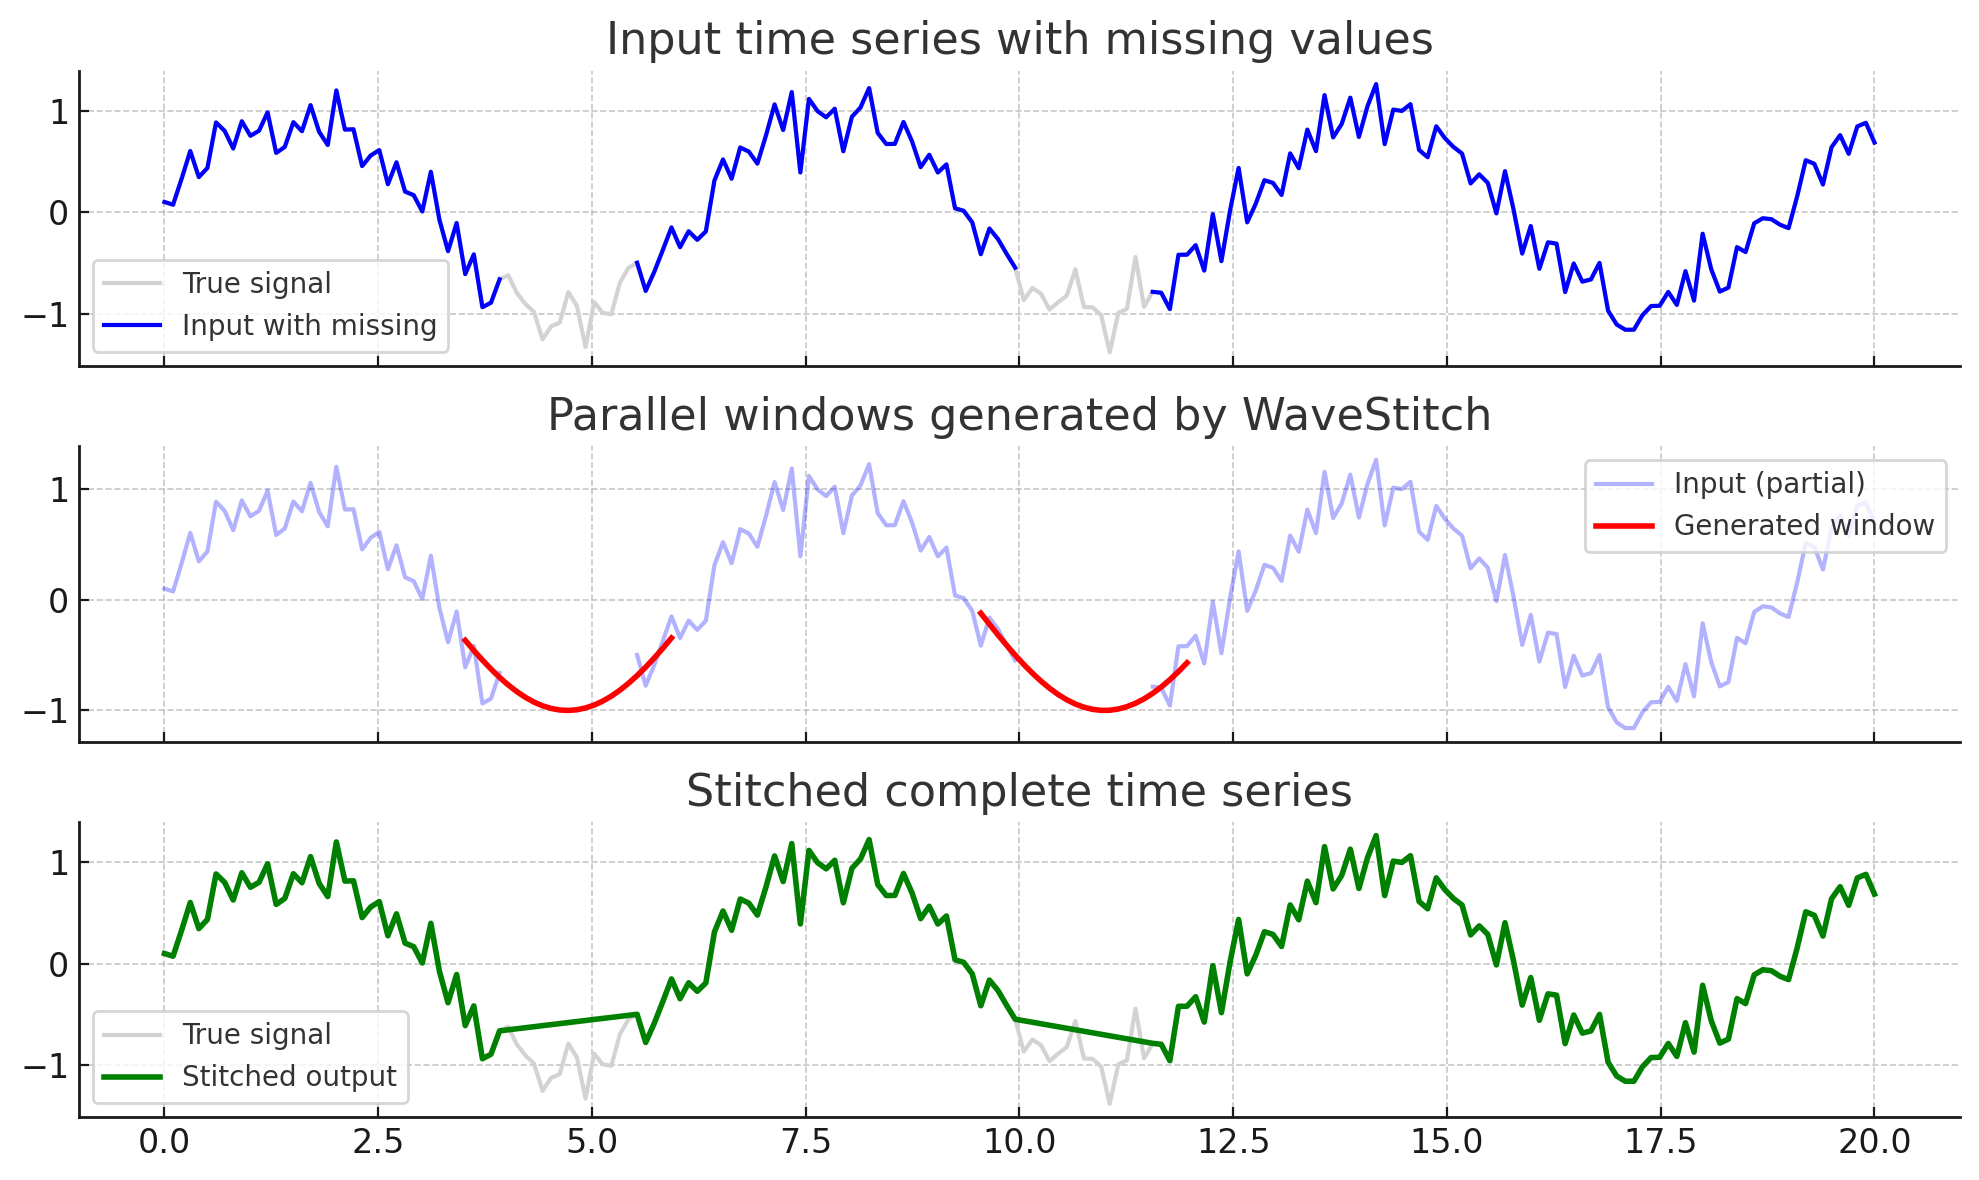
\includegraphics[width=0.75\textwidth]{images/esempio_wavestitch.png}
    \caption{Conceptual diagram of how WaveStitch works (own elaboration): (top) input with missing values; (center) windows generated in parallel; (bottom) complete series obtained through \textit{stitching}.}
    \label{fig:wavestitch_schema}
\end{figure}


% ------------------------
\section{Machine learning in relation to this work}

\textbf{Machine learning} (ML) is now one of the most powerful tools for analyzing and modeling complex data.  
In a nutshell, I would say that the idea behind ML is to train algorithms capable of learning rules and patterns directly from data, without the need for explicit programming.  

% ----------------------
\subsection{Supervised vs. Unsupervised Learning}

I would say that the work I am presenting straddles two classic ML paradigms:

\begin{itemize}
    \item \textbf{Supervised Learning:} there is a model that is trained on a labeled dataset (each instance associated with the corresponding class). This means that for each example in the training dataset, there is a corresponding label or desired result. The goal of the model is to learn a function that maps inputs to the correct outputs, so that it can make accurate predictions on new, unseen data.  

    \item \textbf{Unsupervised learning:} when data does not have explicit labels, classes are not known a priori. In this case, the goal is to identify latent structures or statistical relationships, as occurs when we cluster data.  
\end{itemize}
Although the \emph{WaveStitch} model is a conditional generator, it works in a manner similar to \emph{unsupervised learning}, as it learns the distribution of data without the need for explicit labels, but uses masks and conditional constraints to guide generation.

% ----------------------
\subsection{Mathematical example}

A simple example of a supervised learning model is \textbf{linear regression}, which aims to estimate a linear relationship between a set of independent variables and a dependent variable.  
In compact form, the model can be expressed as:

\[
\hat{y} = w_0 + w_1 x_1 + w_2 x_2 + \dots + w_n x_n,
\]

where \( \hat{y} \) represents the predicted value, \( x_i \) the input variables, and \( w_i \) the associated weights (or coefficients), including the intercept \( w_0 \).  
The model parameters are estimated by minimizing a loss function, typically the \emph{mean squared error} (MSE), defined as:

\[
MSE = \frac{1}{n} \sum_{i=1}^{n} (y_i - \hat{y}_i)^2,
\]

where \( y_i \) is the observed actual value and \( \hat{y}_i \) the corresponding model prediction.  
Minimizing the MSE allows us to obtain the coefficients \( w_i \) that best approximate the relationship between the variables, minimizing the overall difference between actual and estimated values.

\medskip

\noindent
\textbf{WaveStitch}, on the other hand, does not seek a deterministic function \( f(x) \), but learns to generate samples from a probabilistic distribution \( p(x) \), through a process of \emph{diffusion} and subsequent \emph{denoising}~\cite{wavestitch}.  
\emph{Machine learning} therefore acts as a methodological glue between raw data management and the application of advanced generative models, but without adequate \emph{preprocessing} and preliminary statistical analysis, as I will show in the following chapters, even a powerful model such as WaveStitch would fail to produce consistent and reliable results~\cite{bishop2006pattern,hastie2009elements}.
% --------------------------------

\section{Data Clustering in Artificial Intelligence}

\textbf{Clustering} is an \emph{unsupervised learning} technique that allows a set of data to be divided into homogeneous groups, called \emph{clusters}, so that observations belonging to the same group are \emph{similar} to each other, while those belonging to different groups are \emph{dissimilar}~\cite{jain2010data}.  
Clustering is a fundamental tool for exploring and understanding data, as it allows latent structures, recurring patterns, and hidden relationships to be identified without resorting to predefined labels.

\subsection{Basic principles}

Given a set of $n$ objects and a predetermined number $k \leq n$ of clusters to be created, the goal of clustering is to organize the data into $k$ partitions such that:
\begin{itemize}
  \item objects within the same cluster are \textit{similar} to each other;
  \item objects belonging to different clusters are \textit{dissimilar}.
\end{itemize}
In other words, clustering can be considered a form of \emph{lossy data compression}, in which each group represents a collective abstraction of multiple observations.

\subsection{k-Means algorithm}

During my Information Systems course, I learned about various algorithms such as \textbf{k-medoids} and \textbf{k-modes}, but for this work I wanted to choose one of the most widespread and widely used as a tool and subject of study: \textbf{k-Means}. I will explain how it works below.  
The algorithm operates according to an iterative partitioning approach, in which each data point is assigned to the cluster whose \emph{centroid}—i.e., the average of the points belonging to that cluster—is closest.  

The process can be described as follows:
\begin{enumerate}
  \item $k$ initial centroids are randomly selected from the dataset.
  \item Each point is assigned to the cluster with the closest centroid (usually according to Euclidean distance).
  \item The centroids are updated as the average of the points assigned to each cluster.
  \item Steps (2)–(3) are repeated until convergence, i.e., until the assignments do not change or a maximum number of iterations is reached.
\end{enumerate}

Formally, the algorithm minimizes the following objective function:

\[
J = \sum_{i=1}^{k} \sum_{x \in C_i} \| x - \mu_i \|^2
\]

where $C_i$ represents the $i$-th cluster and $\mu_i$ its centroid.  
The aim is therefore to minimize the overall distance of the points from their respective centroids, obtaining compact and well-separated clusters.

\subsection{Advantages and limitations}

The k-Means method has several advantages:
\begin{itemize}
  \item it is simple to implement and conceptually intuitive;
  \item it is scalable and efficient even on large datasets, with complexity $O(nkt)$, where $n$ is the number of objects, $k$ is the number of clusters, and $t$ is the number of iterations;
  \item it works well when clusters are compact and separable.
\end{itemize}

However, it also has some limitations~\cite{jain2010data}:
\begin{itemize}
  \item it requires specifying the number $k$ of clusters in advance;
  \item it is sensitive to the choice of initial centroids and can converge to local optima;
  \item it is not suitable for non-convex clusters or clusters with very different densities;
  \item it is influenced by \emph{outliers}, which can significantly alter the position of the centroids.
\end{itemize}

\subsection{Convergence and variants}

The k-Means algorithm guarantees convergence in a finite number of steps, since there is a finite number of possible data partitions and each iteration reduces (or keeps constant) the objective function $J$. In the next chapter I will talk about the Wavestitch Paper. 
